\chapter{АНАЛІЗ ЗАДАЧІ ПЛАНУВАННЯ У ХМАРНОМУ СЕРЕДОВИЩІ}

% !TEX root = ../thesis.tex

\section{Планувальники у розподілених обчисленнях}

Планувальники в загальному поділяються на два типи: статичні та динамічні. Статичні мають певне правило розподілу задач на обчислювальні вузли та правило не змінюється під час роботи планувальника. Динамічні планувальники в свою чергу можуть адаптуватися під час роботи та змінювати стратегії планування. Хоч динамічні планувальники і здаються більш універсальними, проте вони дуже складні для аналізу та часто розробляються з метою оптимізації певного параметра.

Основною метою планування є розподіл виконання задач, які надсилають користувачі, між обчислювальними вузлами. Планувальник формує чергу виконання задач, та визначає яку задачу на якому вузлі стартувати. Частіше за все користувачів хвилює лише мінімізація часу завершення деякої відправленої множини задач у хмару.

Структура хмари у загальному випадку описується за допомоги таких сутностей як:
\begin{itemize}
	\item брокер
	\item планувальник
	\item дата центр
	\item хост
	\item віртуальна машина
\end{itemize}

На Рис. \ref{fig:cloud_representation} проілюстрована структура простої хмарної системи з одним сервером. Брокер являється посередником між користувачем та хмарою і саме він формує запити до хмари на виконання задач та отримує результати їх виконання. Планувальник отримує задачі від брокерів різних користувачів та має свою певну стратегію розподілу черги задач, саме він керує дата центрами. Дата центри це несамостійні сутності і повністю керовані планувальниками. Їх основна мета - надавати обчислювальні вузли, запускати задачі по команді від планувальника та віддавати результати. Також у випадку динамічної хмари по певним запитам вони можуть збільшувати чи зменшувати кількість обчислювальних вузлів у мережі.

\begin{figure}[H]
	\centering
	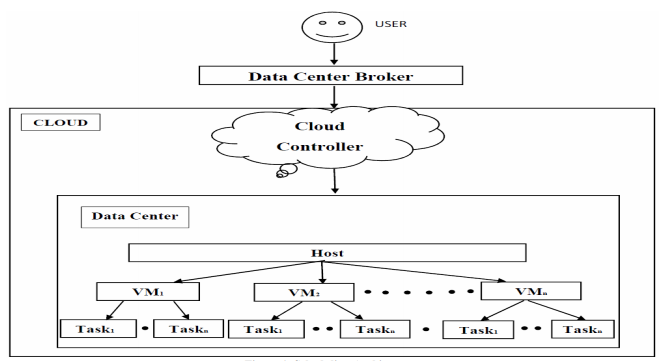
\includegraphics[width=\textwidth]{task_analysis/img/cloud_representation}
	\caption{Ілюстрація структури хмарної ОМ}
	\label{fig:cloud_representation}
\end{figure}

Віртуальна машина - це окремий обчислювальний вузол, який вміє лише отримувати вхідні дані, виконувати задачу та відправляти результат у дата центр. Часто буває таке, що декілька віртуальних машин працюють на одній фізичній машині, це звичайне явище, яке обумовлене тим, що дешевше на сервері із 64 чи 128 обчислювальними ядрами встановити багато віртуальних машин по 4 обчислювальних ядра. Часто користувачами не потрібні багатоядерні машини.

Існує дві політики планування: space shared та time shared Рис. \ref{fig:time_space_shared}. У політиці space shared задачі у черзі розділяють між собою логічні ядра процесора обчислювального вулза і у випадку якщо усі ядра зайняті, то задач чекає звільнення ядра. Саме ця політика і використовується для тестування алгоритмів планування оскільки у випадку коли обчислювальні вузли мають лише одне ядро процесора, задачі виконуються послідовно від початку до кінця. Найпростіший алгоритм, який можна зустріти разом з політикою space shared - first come first served (FCFS).

\begin{figure}[H]
	\centering
	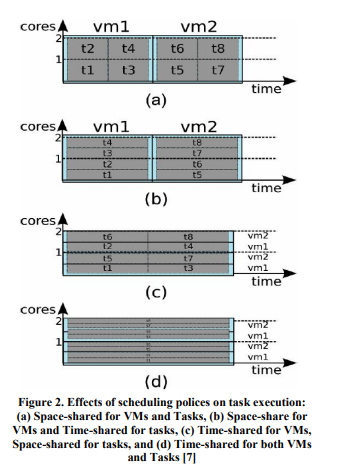
\includegraphics[width=\textwidth]{task_analysis/img/time_space_shared}
	\caption{Ілюстрація планування задач для time та space shared }
	\label{fig:time_space_shared}
\end{figure}


Етапи роботи space shared політики:
\begin{itemize}
	\item[Крок 1] Формується черга задач.
	\item[Крок 2] Запланувати виконання наступної задачі із черги.
	\item[Крок 3] При завершенні задачі відправити результат.
	\item[Крок 4] Якщо черга непорожня, то повернутися на крок 2.
	\item[Крок 5] Кінець.
	\item[***] Нові отримані задачі додаються до черги та очікують свого запуску свого виконання.
\end{itemize}

Time shared політика в свою чергу означає що задачі у черзі розділяють між собою процесорний час. Тобто не обчислювальні ресурси, а проміжки часу які будуть витрачені на виконання кожної із задач. Усі задачі в черзі стартують в один і той самий час. Задача планувальника в цьому випадку - вирішувати коли потрібно призупинити виконання одної задачі та стартувати чи продовжити виконання іншої задачі. На перший погляд ця політика значно краща оскільки дозволяє виконувати набір задач поступово, проте час переключення від одної задачі до другої також потрібно враховувати. А також щоб стартувати усі задачі потрібно мати вхідні дані для усіх задач, що також не завжди зручно. Разом з цією політикою часто можна зустріти посилання на алгоритм планування Round Robin.

Етапи роботи time shared політики:
\begin{itemize}
	\item[Крок 1] Формується черга задач.
	\item[Крок 2] Усі задачі запускаються одночасно у режимі переключення між задачами за правилом, яке визначає планувальник.
	\item[Крок 3] Кінець.
	\item[***] Нові отримані задачі додаються до черги та зразу запускаються і працюють у режимі спільного використання процесорного часу.
\end{itemize}

З цього можна зробити висновки, що space shared політика задає послідовне виконання задач обчислювальними вузлами, а time shared - паралельне. Time shared політика рідко використовується у багатопроцесорних середовищах коли ОВ розташовані далеко один від одного. Також вона потребує спеціальної технології переключення між задачами, яка забезпечить дуже швидке переключення між задачами. Але такі технології зазвичай спеціалізовані і непридатні для виконання будь-яких задач.

У цій роботі використовується політика space shared оскільки саме вона передбачає виконання лише одної задачі на обчислювальному вузлі у кожен момент часу.



\section{CloudSim як засіб для симуляції хмарних обчислень}

Останнім часом технологія хмарних обчислень виникла як провідна технологія для забезпечення надійних, безпечних, відмовостійких, стійких та масштабованих обчислювальних послуг, які представлені як програмне забезпечення, інфраструктура або платформа як послуги (SaaS, IaaS, PaaS). Більше того, ці послуги можуть бути запропоновані в приватних центрах обробки даних (приватні хмари), можуть бути комерційно запропоновані для клієнтів (загальнодоступні хмари), або можливо, що як державні, так і приватні хмари об'єднуються в гібридні хмари.

Ця вже широка екосистема хмарних архітектур, разом із зростаючим попитом на енергоефективні ІТ-технології, вимагає своєчасних, повторюваних та контрольованих методологій для оцінки алгоритмів, програм і політики до фактичного розвитку хмарних продуктів. Оскільки використання реальних тест-сейфів обмежує експерименти до масштабу тест-сейфів і робить відтворення результатів надзвичайно важким завданням, альтернативні підходи для тестування та експериментів сприяють розробці нових технологій Cloud.

Підходящою альтернативою є використання інструментів моделювання, що дають можливість оцінити хмарну систему перед розробкою програмного забезпечення в середовищі, де можна відтворити тести. Зокрема, у випадку обласного обчислення, коли доступ до інфраструктури здійснює платежі в реальній валюті, підходи на основі моделювання дають значні переваги, оскільки це дозволяє Cloud клієнтам протестувати свої послуги в повторимому та контрольованому середовищі безоплатно, а також настроювати продуктивність вузькі місця до розгортання на реальних хмарах. На стороні постачальника, симуляційні середовища дозволяють оцінити різні види сценаріїв лізингу ресурсів при різному розподілі навантаження та ціноутворення. Такі дослідження могли б допомогти постачальникам оптимізувати вартість доступу до ресурсів з упором на підвищення прибутку. За відсутності подібних імітаційних платформ, клієнти Cloud і постачальники повинні спиратися або на теоретичні та неточні оцінки, так і на підходи щодо спроб і помилок, які призводять до неефективної ефективності обслуговування та отримання доходу.

Основна мета цього проекту полягає у забезпеченні узагальненої та розширюваної системи моделювання, яка дозволяє безперешкодно моделювати, моделювати та експериментувати з розвиваються інфраструктурою Cloud Computing та додатковими службами. Використовуючи CloudSim, дослідники та розробники на базі промисловості можуть зосередити увагу на конкретних проблемах дизайну систем, які вони хочуть досліджувати, не занепокоєні деталями низького рівня, пов'язаними з інфраструктурою та службами Cloud.

\subsection{Сильні сторони}

CloudSim фреймворк \cite{CloudSim} достатньо широко охоплює хмарні системи та їх внутрішню структуру. Саме за його допомоги можна перед проектуванням хмарної інфраструктури спочатку провести симуляції та перевірити адекватність спроектованої архітектури мережі.

Пакет працює на базі подій і усі процеси, що моделюються за допомогою CloudSim, реєструються як події. Також як і запит на створення обчислювального вузла, запит на виконання задач та інші. Це дозволяє додавати нові елементи у симуляційну систему без змін в існуючих файлах, потрібно лише створити свою власну подію та додати її обробку до сутностей, в яких ця подія відбувається. Додаваня обробки події часто виконується через наслідування від основного об'єкта та імплементації метода "processEvent".

Така система дуже гнучка та дозволяє швидко написати свою власну симуляцію.

\subsection{Слабкі сторони}

СПЗ CloudSim написане на мові програмування Java та непридатне для моделювання ситуацій з великою кількістю задач. Це одна із проблем, яка і привела до написання власної упрощеної версії СПЗ на мові C++, яка скоритила час симуляцій майже в 50 разів у порівнянні з модифікованою версією СПЗ, яка була написана на базі CloudSim та була майже у 150 разів швидшою за звичайну версію.

Також сама по собі мова Java неадекватно працює у випадку коли потрібно швидко створики велику кількість малих об'єктів, провести з ними певні операції та видалити.

Наприклад, для симуляції множення двох матриць $N*N$ та $N*N$, при розмірі розрізання $n=1$ для одного користувача буде створено $N*N$ задач множення підматриць розмірів $1*N$ та $N*1$. Звісно цей приклад не має сенсу оскільки розрізання $n=1$ скоріше за все не ефективне, проте сама неможливість його змоделювати для $N=5000$ вважається великим недоліком, оскільки поставивши $N=50000$ та $n=10$ отримаємо таку ж саму кількість задач, і лише на їх створення на мові Java витрачається більше 5 секунд. У той час как симуляція, написана на мові С++ дозволяє за ці 5 секунд провести 2 симуляції з такими ж параметрами.

Також слід зазначити, що першою спробою написання симуляції для цієї роботи було саме використання CloudSim. Проте під час розробки програми доводилось дуже довго вивчати документацію і виправляти деякі внутрішні недоліки. Наприклад, у системі була знайдена проблема, що велика кількість малих задач оброблялась повністю і обривалась у випадковому місці. Це пов'язано з тим, що система не розроблялась з метою проведення важких симуляцій.

Також під час проведення симуляцій на виправленій версії системи було помічено дуже повільну швидкість симуляцій для великої кількості задач. Було знайдено 2 основні точки, які сильно сповільнювали програму та виправлені. Одна із правок дала пришвидшення симуляцій приблизно у 50 разів, а друга ще у приблизно 100 разів. Проте навіть з цими правками симуляції проходять значно повільніше за написаний нами самуляційний пакет.

\subsection{CloudSim Plus}

CloudSim Plus \cite{CloudSimPlus} це фреймворк, що є удосконаленою версією CloudSim та все ще розвивається, на відміну від свого батька, який не має оновлень з 2016 року. Оскільки пакет розробляється великою кількістю людей у їх вільний час, то довіра до нього сильно падає. Немає ніякого контролю якості системи, особливо ігнорується швидкодія. Також цей пакет може містити помилки у коді, які виправити сторонньому користувачу буде дуже важко, оскільки для цього протрібно знати та розуміти архітектуру саме цього пакета.

Проте саме цей пакет дозволяє проводити симуляції паралельно і на комп'ютерах з декількома ядрами можна отримати пришвидшення набору симуляцій за рахунок паралельного їх запуску. Саме це і було зроблено у першій версії симуляційного пакету. Але швидкодії всеодно було недостатньо, оскільки бажаним результатом було отримати симуляційну систему, яка швидко зможе проводити симуляції усіх можливих комбінацій стратегій двох гравців. І навіть для розміру матриць 1000 симуляція усіх комбінацій проходила більше години

\section{Аналіз існуючих робіт}

У роботі \cite{AppSelAlgoFEffResProvInCloud} проведений короткий аналіз стратегій виділення ресурсів типів Min-Min та Max-Min. Також у цій роботі занадто проста схема задач, складність обчислень прямо пропорційна розмірам файлів, що буває дуже рідко для трудоемних задач. Ця робота проводить симуляції, в яких кількість задач не більше 10 та всього 2 обчислювальних вузла. Проте вони запропонували алгоритм вибору, який покращує звичайну реалізацію стратегії виділення ресурсів. Також у цій роботі був використаний пакет CloudSim як основний засіб для аналізу та перевірки теорії.

Також цікавою роботою є використання теорії керування з метою мінімізації часу на виконання задачі заданого набору задач \cite{Prasanna1991GeneralisedMS}. У цій роботі використовується time shared політика планування та динамічне переключення між виконанням задач. Для цього використовується теорія оптимального керування, яка керує кількістю часу, яка надається для задачі у наступній ітерації. Також доведена еквівалентність задачі планування і задачі оптимального управління часом.

Проблема ефективного множення великих матриць також розглянута у \cite{PushingTheBoundsOfMatrixMatrix}. У цій роботі розглядають більш стандартизовану операцію над матрицями: $C := A*B + C$. Ця операція є основною у бібліотеках стандарту BLAS (Basic Linear Algebra Subprograms), яка в них називається GEMM (General Matrix Multiply) та описується як $C = \alpha A*B + \beta C$. Робота базується в першу чергу на \cite{IOComplexityMatrixMatrix} та \cite{Irony}, я яких проводиться аналіз складності вводу та виводу у випадку множення матриць і також можливі оптимізації, які можна застосувати у розподіленому середовищі з метою зменшення затрат на операції передачі даних. Ця проблема також випливає і у нашому дослідженні, оскільки показано, що надлишковість передачі даних при розбитті матриць на блоки дуже швидко зростає, проте найбільш оптимальними розбиттями є саме розбиття на малі блоки так як вони мінімізують простоювання вузлів при завершенні виконання блоку задач. Дослідження у роботі виконані саме для випадку блочного розбиття матриць і не підходять для паралельної версії алгоритма Штрассена.

Одна з свіжих робот на тематику ефективного множення матриць це \cite{CodedHeterogeneousMatrixMatrix}. В роботі розглядається операція $y:=Ax$ для матриці $A \in \mathbb{R}^{m*n}$ та вектора $x \in \mathbb{R}^{n}$ як частковий випадок множення двох матриць. Побудована модель обчислень також включає дві схеми: Uncoded Load Balanced (ULB) та Coded Equal Allocation (CEA). Особливістю роботи є оцінка оптимальної конфігуляції обчислювального середовища на базі Amazon AWS завдяки побудові моделі. Знаходиться компроміс між вибором набору кластерів із заплопонованих тарифних планів та швидкістю виконання операцій. Для пошуку оптимальної конфігурації запропонований еврестичний пошук. На основі цієї роботи була запропонована покращена схема кодування та проведені порівняння з існуючими \cite{CodedHeterogeneousMatrixMatrix2}.



\section*{Висновки до розділу}
\addcontentsline{toc}{section}{Висновки до розділу}

У цьому розділі було розглянуто структуру принципи роботи об'єкта дослідження - хмачного середовища. ХС у наші дні це дуже поширейний інструментр для виконання задач користувачів будь-якої складності та вважається, що воно замінить у певному сенсі домашні обчислювальні машини.

Розглянуті популярні засоби для симуляції хмарного середовища - CloudSim, CloudSim Plus та GridSim. Ці засоби дуже популярні та часто використовуються у бакалаврських чи магістерських роботах для тестування спроектованих планувальників. Ці СПЗ не підходять для даної роботи оскільки вони написані на мові Java та мають низьку швидкодію у випадку великої кількості задач.

Із огляду літератури можна зробити висновнки, що тема актуальна і нові дослідження проводяться навіть для таких простих задач як множення матриць чи добутку матриці на вектор.